\section{Method: a dense localization prior}
\label{sec:method}

\begin{figure*}[t]
\centering
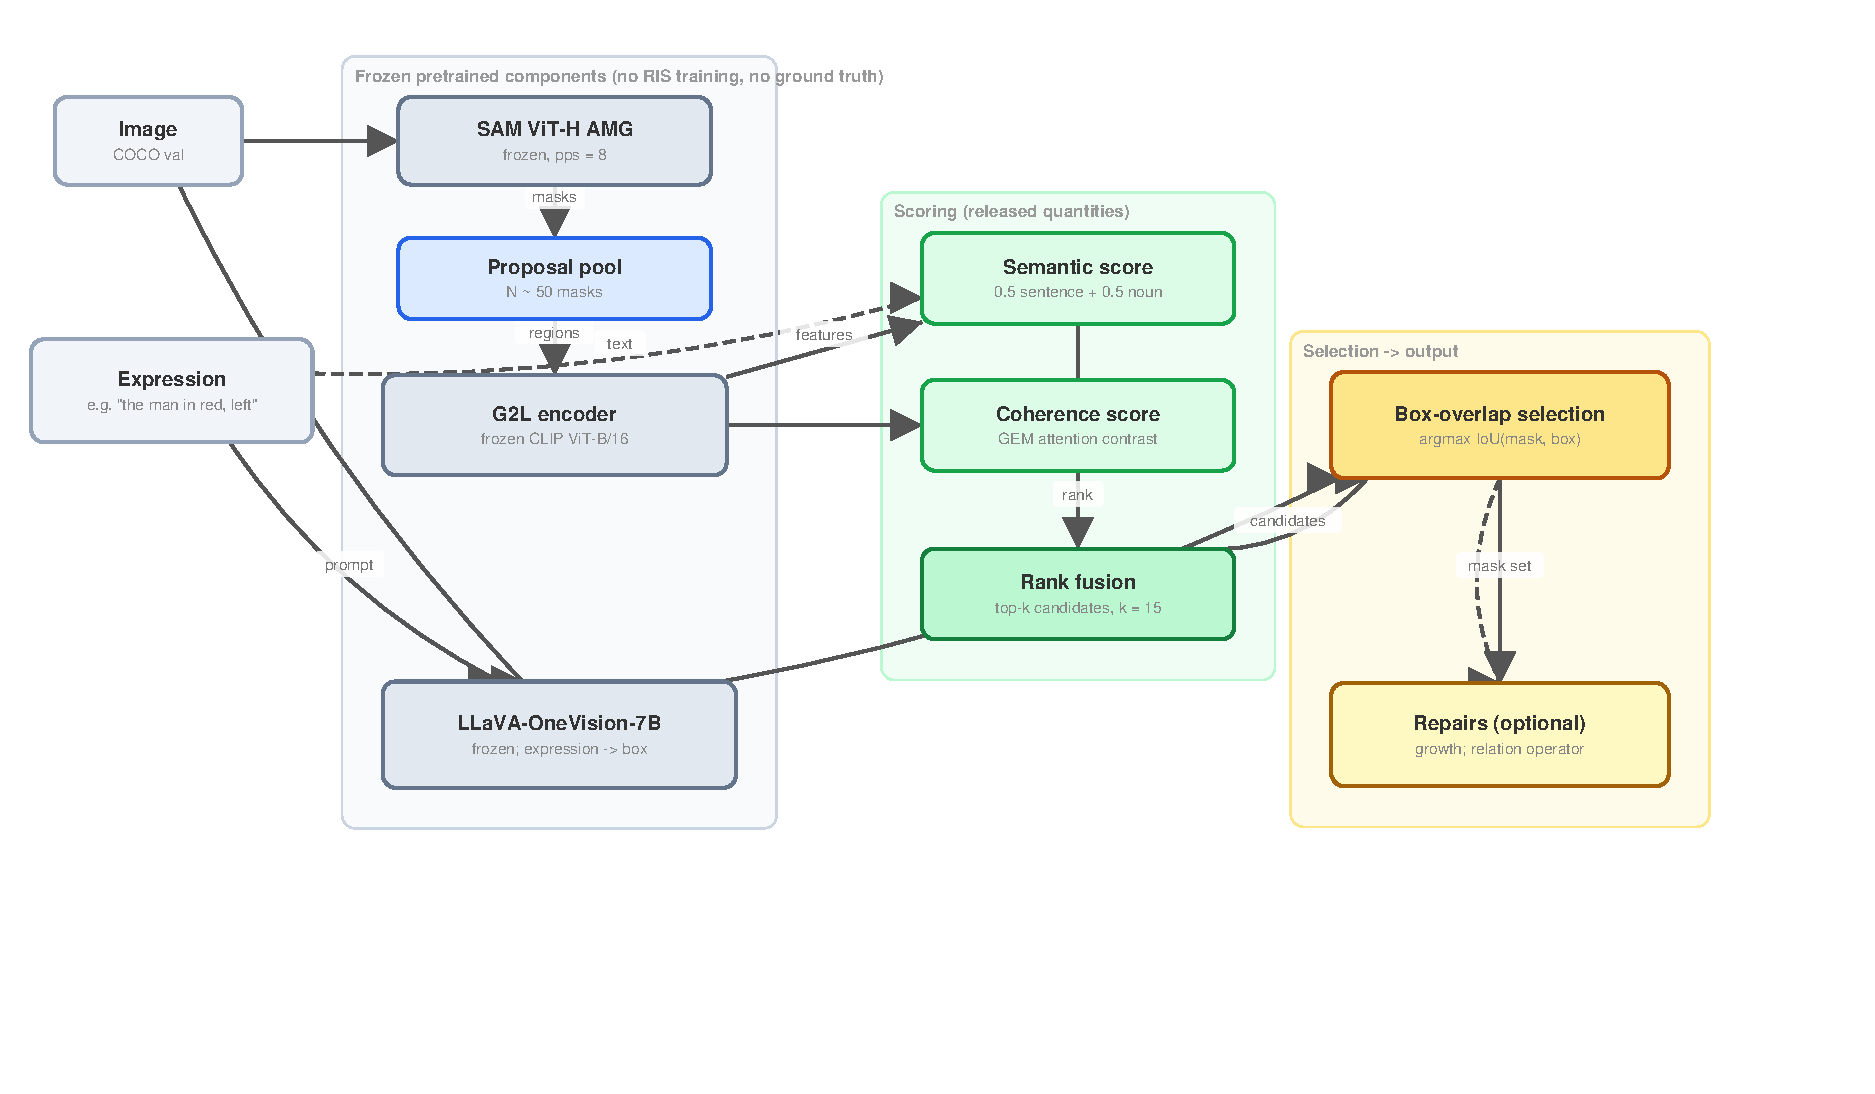
\includegraphics[width=0.98\textwidth]{figures/architecture.pdf}
\caption{The shipped pipeline. Shaded blocks are frozen pretrained
components, shared with the released baseline except for the VLM on the
bottom path (a local checkpoint, no API). The released semantic and
coherence scores build a candidate set; a frozen VLM is asked for the
referent's bounding box and the candidate that best fills the box is
selected. Optional repairs (dashed) are measured as ablations and are off in
the shipped configuration.}
\label{fig:arch}
\end{figure*}

\subsection{Setup and notation}
We build on the released HybridGL pipeline~\cite{hybridgl2025}, the strongest
training-free referring segmentation family with runnable code. For an image
$I$ and expression $T$ it produces a pool of $N$ masks $M=\{m_1,\dots,m_N\}$
with SAM ViT-H~\cite{kirillov2023sam} (automatic mask generation,
\texttt{points\_per\_side}{}$=8$), extracts a G2L region feature for every
mask with a frozen CLIP ViT-B/16 backbone (the masked region, and the image
with its complement blurred), and computes two released quantities: a
\emph{semantic score} $S^{\mathrm{dec}}_i$ (cosine of the region feature with
the $0.5$ sentence $+$ $0.5$ noun-phrase text ensemble) and a \emph{coherence
score} $S^{\mathrm{coh}}_i$ (the GEM~\cite{hybridgl2025} attention contrast inside
minus outside the mask). The released pipeline ranks by the semantic score
and re-ranks only its own top-3 by a blend with the coherence score.

\subsection{The missing input is localization}
\label{sec:why}
Our diagnosis (Section~\ref{sec:diagnosis}) shows the pool is not the
bottleneck: for \oracleHitPct\,\% of RefCOCO val expressions it already
contains a mask with $\mathrm{IoU}\ge0.5$, and the best achievable single
choice sits at \oracleRefcoco\,mIoU. What the pipeline lacks is a signal that
says \emph{where the referent is} when the expression is descriptive rather
than spatial. Both released scores are region--text similarities: they
compare a whole-region embedding with a whole-sentence embedding, so on
RefCOCO+ --- whose expressions are constructed without location words --- the
pipeline returns the wrong instance for most of its errors, and replacing the
encoder with a stronger one (SigLIP-so400m) does not help
(\S\ref{sec:ablations}): the deficit is instance-level grounding, not
embedding quality.

\subsection{Dense box prior from a frozen VLM}
\label{sec:boxprior}
We therefore add a single off-the-shelf component: a frozen vision-language
model, asked in natural language for the referent's bounding box. We use
LLaVA-OneVision-7B~\cite{li2024llavaov}, queried locally --- no external API, no
key, no network at inference --- with the prompt
\begin{quote}\small
``Locate the \{expression\} in this image. Reply with ONLY the bounding box
as [x0,y0,x1,y1] in pixel coordinates \dots, or the single word none if it
does not appear in the image.''
\end{quote}
parsing the first four numbers and treating values $\le 1.5$ as normalised
coordinates. Crucially we pass the \emph{full referring expression}, not a
parsed noun phrase: on the held-out split this single choice is worth
$+13.4$/$+10.6$/$+11.6$ mIoU over the noun-phrase prompt
(Table~\ref{tab:studies}), because for RefCOCO+ and RefCOCOg the
discriminating information lives in the attributes and relations, not in the
head noun.

Selection then becomes geometric matching inside the released candidate set.
Let $B$ be the VLM box and let
$\mathcal{C}=\operatorname{top-}k_i\big(\operatorname{rank}(S^{\mathrm{dec}}_i)
+ \gamma\,\operatorname{rank}(S^{\mathrm{coh}}_i)\big)$ be the top-$k$ masks
by rank fusion of the two released scores, with $k,\gamma$ chosen on the
held-out split. The output is
\begin{equation}
\label{eq:select}
j^\star = \argmax_{i \in \mathcal{C}} \; \mathrm{IoU}(m_i, B),
\qquad
\hat{M} = \begin{cases} m_{j^\star} & B \neq \texttt{none}\\ \emptyset & B = \texttt{none}\end{cases}
\end{equation}
the candidate that best fills the region the VLM points at. The released
scores are still used --- but only to keep the box match away from same-class
distractors: without the candidate restriction the box prior alone is worse
(\S\ref{sec:ablations}).

Repairs from our earlier diagnosis remain available and are measured
separately: \emph{containment growth} (replace the selection by its smallest
strict container in the pool) and the \emph{relation-gated operator} (for
parsed spatial expressions, re-rank the category-score top-$8$ by the
coherence score within the side selected by the relation). Both are
\emph{off} in the shipped configuration --- the VLM prior subsumes them ---
and appear as ablations.

\subsection{Set-valued extension}
\label{sec:setvalued}
For benchmarks whose targets may be multiple or absent (gRefCOCO), we split
the expression on \texttt{and}/\texttt{or}/``,'', query one box per clause,
select one candidate per clause with Eq.~\ref{eq:select}, and return the
union; if every clause answers \texttt{none} the prediction is empty. This
keeps the same frozen components and turns ``no such object'' into a
\emph{decided} output rather than a score threshold. Section~\ref{sec:gref}
reports what this buys and why the remaining gap on that benchmark is a
property of the comparison class, not of the selector.

\subsection{What is and is not trained}
Nothing is trained, fine-tuned, or adapted on referring data: SAM, CLIP, GEM
and the VLM are used frozen, exactly as released. The only fitted quantities
are five scalars (candidate base, $k$, $\gamma$, overlap mode, growth
flag) selected by Optuna on a held-out split built from RefCOCO-family
\emph{train} references; the official validation and test splits are never
used for tuning (\S\ref{sec:studies}). The VLM is a local checkpoint
(15\,GB) served at $0.6$--$1.8$\,s per expression on one RTX 4090; we also
ran it 8-bit quantised ($9.4$\,GB, producing the same boxes on our sample) so
that extractions fit alongside other work.
